\documentclass[aps,prl,10pt,twocolumn,superscriptaddress,showpacs]{revtex4-1}
\usepackage{titlesec}
\usepackage{hyperref}
\usepackage{graphicx}
\usepackage{amsfonts,amsmath,amssymb,bm,bbm}
\usepackage{color}
\usepackage{todonotes}

\usepackage{caption}
\usepackage{subcaption}

\hypersetup{
    pdfnewwindow=true,      % links in new window
    colorlinks=true,       % false: boxed links; true: colored links
    linkcolor=blue,          % color of internal links
    citecolor=blue,        % color of links to bibliography
    filecolor=blue,      % color of file links
    urlcolor=blue        % color of external links
}

\titleformat{\section}[runin]
  {\normalfont\bfseries}{\thesection}{1em}{}[:]
\titlespacing*{\section}{0cm}{2em}{1em}
\titleformat{\subsection}[runin]
  {\normalfont\itshape}{\thesubsection}{1em}{}[:]
\titlespacing*{\subsection}{1cm}{2em}{1em}

\newcommand{\bvec}[1]{\mathbf{#1}}
\newcommand{\units}[1]{\,\mathrm{#1}}
\newcommand{\comments}[1]{}

\graphicspath{{../img/}}

\begin{document}

\title{The Doppler effect on indirect detection of decaying dark matter}
\author{Devon Powell}
\email{dmpowel1@stanford.edu}
\author{Ranjan Laha}
\email{rlaha@stanford.edu}
\author{Tom Abel}
%\email{tabel@stanford.edu}
\affiliation{Kavli Institute for Particle Astrophysics and Cosmology (KIPAC),
	\\ Department of Physics, Stanford University, Stanford, CA 94305, USA}
\affiliation{SLAC National Accelerator Laboratory, Menlo Park, CA 94025, USA}
\date{\today}

\begin{abstract}
\cite{speckhard2016}
\end{abstract}

%\pacs{95.35.+d, 13.35.Hb, 14.60.St, 14.60.Pq}
% 95.35.+d Dark matter
% 13.35.Hb Decays of heavy neutrinos
% 14.60.St Non-standard-model neutrinos, right-handed neutrinos, etc.
% 14.60.Pq Neutrino mass and mixing 

\maketitle


% % % % % % % % % % % INTRODUCTION % % % % % % % % % % % % % % % % % % % % % %
\section{Introduction}
\label{sec:Introduction}

The search for the particle properties of dark matter is one of the most important research avenues\,\cite{Jungman:1995df,Bertone:2004pz,Strigari:2013iaa}.  The ``weak" interactions experienced by the dark matter particle complicates these searches.  Despite decades of multi-pronged searches, we have not yet identified the dark matter particle\,\cite{Bertone:2016nfn}.  One of the most important ways to search for dark matter particles is indirect detection\,\cite{Klasen:2015uma}.

Due to the enormous astrophysical background, many anomalous signals have been interpreted as a  dark matter signal\,\cite{Abazajian:2014hsa,Daylan:2014rsa,Lee:2015fea,Bartels:2015aea,Bulbul:2014sua,Boyarsky:2014jta,Urban:2014yda}.  Astrophysical sources such as pulsars or atomic lines are diverse enough to mimic a dark matter signal\,\cite{O'Leary:2015gfa,Brandt:2015ula,O'Leary:2016osi,Gu:2015gqm,Phillips:2015wla,Shah:2016efh}.  The separation of signal and background is difficult since one needs to model the background and then find the signal in the same data set.  Distinct kinematic signatures arising from dark matter annihilation or decay are used to separate the dark matter signal from background.  These signatures include monochromatic photons arising from dark matter annihilation or decay.  Past experiences have shown that it is not reliable to only depend on this signature for the identification of a dark matter signal.

In order to better characterize a dark matter signal, Ref.\,\cite{speckhard2016} utilized the superb energy resolution, $\sim \mathcal{O}$(0.1\%), of Hitomi (previously known as Astro-H) to find a new signature.  It was shown that our motion around the Galaxy produces a distinct longitudinal dependence in the dark matter signal --- a signature of Doppler effect.  This new signature is model independent and applicable to any dark matter signal containing a sharp feature.  It is unlikely that baryonic phenomenon can produce such a distinct signature\,\cite{speckhard2016}.

Given the importance of identifying the dark matter particle, it is important to characterize any new model independent signature in detail.  We perform such a study in this work using dark matter only simulations from Ref.\,\cite{mao2015}.  As an example of the dark matter signal, we consider the 3.5 keV line\,\cite{Bulbul:2014sua,Boyarsky:2014jta}.  The status of the 3.5 keV line is controversial\,\cite{Iakubovskyi:2015wma,Jeltema:2015mee,Ruchayskiy:2015onc,Bulbul:2016yop,Aharonian:2016gzq,Hofmann:2016urz,Conlon:2016lxl}.  The malfunctioning of the Hitomi satellite did not permit an observation which would have conclusively tested this signal.  We use future Micro-X observations\,\cite{Figueroa-Feliciano:2015gwa} to demonstrate our technique.  It is expected that Micro-X will have an energy resolution of 3 eV at 3.5 keV\,\cite{Figueroa-Feliciano:2015gwa}, and thus permits dark matter velocity spectroscopy\,\cite{speckhard2016}.  We emphasize that we are using this 3.5 keV signal as a proxy, and that the underlying physics of this work is model independent.  

Any telescope with $\mathcal{O}$(0.1 \%) energy resolution can perform dark matter velocity spectroscopy.  An improvement in the energy resolution is the natural step in the evolution of telescope instrumentation.  This improvement will help in disentangling dark matter signal from background, and improving our knowledge of the astronomical sources.  It is a known technology to build detectors with $\mathcal{O}$(0.1\%) energy resolution, such as INTEGRAL-SPI\,\cite{2003AA} and Hitomi.  Near future instruments like Micro-X\,\cite{Figueroa-Feliciano:2015gwa} and ATHENA\,\cite{Barret:2016ett} will also have a $\mathcal{O}$(0.1\%) energy resolution.

%The decay signal spectral intensity is traditionally defined in terms of a line integral along the viewing direction $\psi$:
%\begin{equation}
%\frac{dI(\psi, E)}{dE} = \frac{\Gamma}{4 \pi m_\chi} \frac{dN(E)}{dE} \int_\phi \rho_\chi(r[s,\phi]) \, ds
%\end{equation}
%where the integral term is the well-known ``J-factor,'' which captures the enhancement of the 
%signal due to substructure.

%The main insight of \cite{speckhard2016} is that for a detector with sufficient spectral
%resolution, the decay spectrum $\frac{dN(E)}{dE}$ can no longer be considered to be independent of
%position.  This is due to Doppler shifting induced by the Sun's motion around the galactic center
%as well as broadening due to the position-dependent velocity dispersion $\sigma(r)$.
%Qualitatively speaking, the observed spectrum is given by the rest-frame decay spectrum
%$\frac{dN(E)}{dE}$ broadened by the dark matter velocity dispersion $\sigma(r)$, shifted by the Sun's velocity 
%relative to the dark halo $\delta E_{MW} = \frac{E v_{MW}}{c}$, and integrated along the line of sight (LOS):

%\begin{equation} \label{eq:analytic}
%\frac{dI(\psi, E)}{dE} = \frac{\Gamma}{4 \pi m_\chi} \int_\phi \rho_\chi(r[s,\phi]) \,
%\frac{d\widetilde{N}(E-\delta E_{MW}, r[s,\phi])}{dE} \, ds
%\end{equation}

%Here, $\frac{d\widetilde{N}}{dE}$ is the rest-frame spectrum broadened by the local
%(position-dependent) velocity dispersion. \cite{speckhard2016} model this as a Gaussian convolution
%with a width dependent on an analytic prescription for $\sigma(r)$.



% % % % % % % % % % % METHODS % % % % % % % % % % % % % % % % % % % % % %
\section{Methods}
\label{sec:methods}
\subsection{Theory}
\label{sec:theory}

For a large field of view instrument\,\cite{Figueroa-Feliciano:2015gwa}:
\begin{eqnarray}
\mathcal{F} = \dfrac{\Gamma}{4\pi \, m_s} \, \int_{\Omega} \int _0 ^\infty d\Omega \, ds \, \rho[r(s, \Omega)] \, .
\label{eq:flux for large FoV}
\end{eqnarray}
We can rewrite Eqn.\,\ref{eq:flux for large FoV} as 
\begin{eqnarray}
\dfrac{d^2 \mathcal{F}}{d\Omega \, dE} =  \dfrac{\Gamma}{4\pi \, m_s} \, \int _0 ^\infty  \, ds \, \rho[r(s, \Omega)] \, \dfrac{dN(E)}{dE} .
\label{eq:double differential for the flux}
\end{eqnarray}

Similar to the previous paper, we can write
\begin{eqnarray}
\dfrac{d \tilde{N} (E, r[s, \Omega])}{dE} =\int dE' \, \dfrac{dN(E')}{dE'} \, G(E - E', \sigma_{E'}) \, ,
\label{eq:formula for modified dNdE}
\end{eqnarray}
where the convolution function $G(E, \sigma_E)$ takes the form of a Gaussian with an width of $\sigma_E = (E/c) \sigma_{v_{\rm LOS}}$.  We assume that $\sigma_{v_{\rm LOS}} \approx \sigma_{v_r}(r[s,\Omega])$.

I will now show the derivation of these formulae.  Let us assume that the velocity distribution is $f(v)$ and the differential spectrum is $dN/dE = \delta (E- E_0)$.  The effect of including this velocity distribution is that it takes the mono energetic spectrum to $\dfrac{d\tilde{N}}{dE} = \delta \left(E - E_0 (1 \pm \dfrac{v_0}{c})\right)$.  From this we can intuitively derive the following formula which is valid for a general $f(v)$:
\begin{eqnarray}
\dfrac{d\tilde{N}}{dE} = \int f(v) \, \dfrac{dN}{dE'} \, G(E, E') \, dv \, dE' \,
\label{eq:step 1}
\end{eqnarray}
where $G(E, E')$ is the convolution function.  To estimate a functional form of $G(E, E')$, we can use the test case $f(v) = \delta (v - v_0)$, and $dN/dE = \delta (E' - E_0)$ to determine $G(E, E') = \delta (E - E' (1 \pm v/c))$.

Let us now consider $f(v) = \dfrac{1}{\sqrt{2\pi} \sigma_v} \, e^{v^2/2 \, \sigma_v^2}$, so that
\begin{eqnarray}
\dfrac{d\tilde{N}}{dE} &=& \int \delta(E' - E_0) \, \dfrac{1}{\sqrt{2\pi} \sigma} \, e^{v^2/2 \, \sigma^2} \, \nonumber\\
&\times& \delta (E - E' (1 \pm v/c)) \, dv \, dE'.
\label{eq:step2}
\end{eqnarray}
We have $\delta (E - E' (1 \pm v/c)) = \dfrac{c}{E'} \, \delta \left(v + c - \dfrac{E}{E'} c \right)$\, .  We can do the integrals to find
\begin{eqnarray}
\dfrac{d\tilde{N}}{dE} =  \dfrac{1}{\sqrt{2\pi}} \dfrac{c}{\sigma_v E_0} {\rm exp} \left( \dfrac{-(E-E_0)^2}{2 E_0^2 \, \sigma_v^2/c^2} \right)
\label{eq:step3}
\end{eqnarray}
which we can compare with a regular Gaussian to derive $\sigma_E = (E/c) \sigma_v$.


\subsection{Simulations}
\label{sec:simulations}

Our main contribution in this paper is to examine the potential of velocity spectroscopy using
N-body simulations, as compared to analytic models using an NFW profile.
To this end, we study a suite of Milky Way analogues run using the L-GADGET cosmology code
(a descendant of GADGET-2, \cite{springel2005}). These are dark-matter-only zoom-in simulations 
run by \cite{mao2015} to study subhalo abundance, and their high resolution and multiple
realizations makes them suitable for our purposes as well. Each halo has $\mathcal{O}(10^7)$
high-resolution particles with a particle mass $m_p=4.0\times10^5\units{M_{\odot}}$ and total 
mass $M_{\mathrm{vir}}\simeq1.2\times10^{12}\units{M_{\odot}}$ (note that here, we quote the masses in physical rather than comoving
units).

\begin{figure}[h!]
\centering
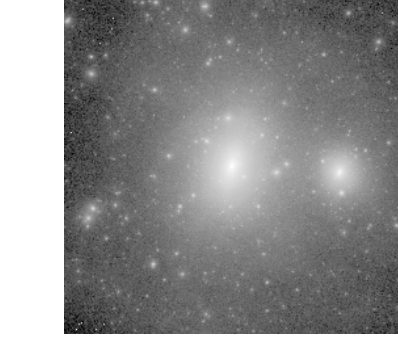
\includegraphics[width=0.9\columnwidth]{halo374.png}
\caption{Halo 374.}
\label{fig:halo374}
\end{figure}

While there are 46 realizations available to us, we focus on one halo (labeled Halo 374, see Figure
\ref{fig:halo374}) in particular. 
This halo is the most spherically-symmetric of the set we studied, with principal axis ratios
$b/a=0.86$ and $c/a=0.73$. Our reason for this choice is that halo triaxility actually plays a role
in the the symmetry of the significance of the observed signal about the Galactic meridian $\ell=0^{\circ}$.
However, the presence of a baryonic disk in the Milky Way tends to make the host
halo more spherical \cite{debattista2008, bryan2013}. As such, we choose to limit ourselves to the more plausible case of
Halo 374, while acknowledging the existence of an effect due to triaxiality. 
We discuss this further in Section \ref{sec:results}.

%\todo{turn halo374 into an illustration of the sampling method rather than just a picture of the halo?}

\subsection{Velocity spectroscopy using simulations}
\label{sec:simulations}

We construct the full
spectral intensity seen by the detector directly from the N-body particles, incorporating Doppler shift
and velocity dispersion in a straightforward and natural way.   This is similar in spirit to both the ``sightline'' method employed by 
\cite{lovell2015} and the velocity distribution function sampling of \cite{mao2013}, both of whom
eschew analytic prescriptions in favor of operating directly on the information available in the
simulation data. 

The procedure for performing velocity spectroscopy on N-body data is relatively straightforward.
The density field in an N-body simulation is effectively a sum of Dirac-$\delta$ functions
$$
\rho(\bvec{x}) = \sum_p\, m_p\, \delta(\bvec{x}-\bvec{x}_p)
$$
where $\bvec{x}_p$ and $m_p$ are the position and mass of particle $p$. Integrating this density over a conical
field of view $\Omega$ then amounts to a sum over all of the particles within that field of view, $p \in
\Omega$, while weighting by the inverse square of the scalar distance to the observer, $r^{-2}_p$. 

Analytically integrating \eqref{eq:flux for large FoV} using this form for the density field yields the
total flux from within the field of view $\Omega$:
\begin{equation} 
	\mathcal{F} = \frac{\Gamma}{4\pi m_s}
	\, \sum_{p \, \in \, \Omega} \, \frac{m_p}{r_p^{2}} 
\end{equation}

Likewise, we can integrate \eqref{eq:double differential for the flux} to sample the Doppler shifted
and broadened observed spectrum:
\begin{equation} \label{eq:discrete}
	\frac{d\mathcal{F}}{dE} = \frac{\Gamma}{4 \pi m_s}\, \sum_{p \, \in \, \Omega}
	\, \frac{m_p}{r_p^{2}} \, \frac{dN[E(1-v_p/c)]}{dE}
\end{equation}
where $v_p$ is the velocity of particle $p$ projected along the line of sight to the observer.

Intuitively, we are ``stacking the spectra'' from the individual simulation
particles, with weights reflecting the $r_p^{-2}$ dependence in the observed flux. One can see that by
considering the LOS velocity of each particle independently, we automatically capture the spectral
convolution introduced by the bulk velocity dispersion. 

We focus here on the special case where
$dN/dE$ is a line. In this case, computing the observed spectrum is then as simple as
building a flux-weighted histogram of the line-of-sight velocities for all particles in the sampling cone,
though as we will see it is easier to forgo binning and compute the line width directly. See Figure
\ref{fig:dfde} for an illustration.

\begin{figure}[h!]
\centering
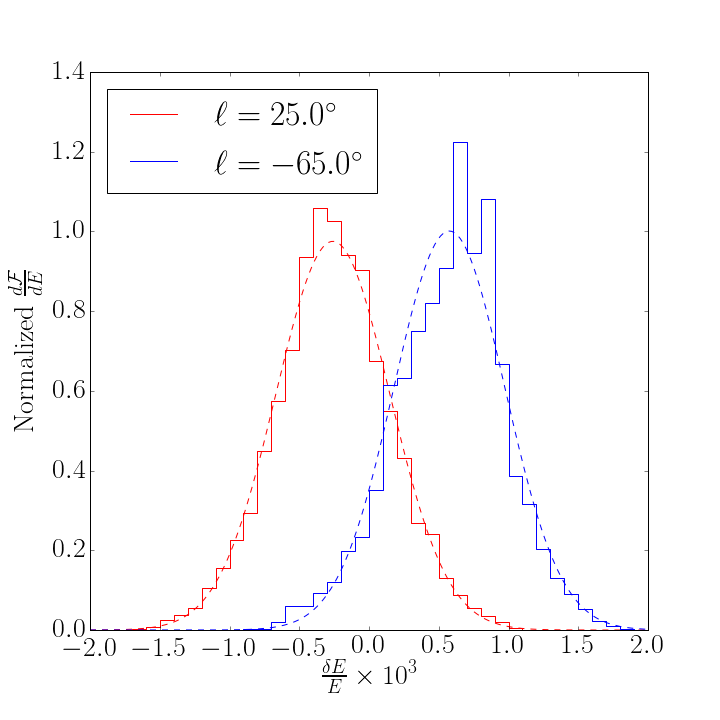
\includegraphics[width=1.0\columnwidth]{dnde_demo.png}
\caption{A comparison of empirical histograms (solid) for the observed line spectrum
	$d\mathcal{F}/dE$ against their Gaussian models (dashed) as computed using \eqref{eq:simcenter} and \eqref{eq:simsigma}.
	These were calculated using Micro-X parameters for galactic latitude $b=25^\circ$ and two galactic
	latitudes $\ell$. These model spectra give a good fit to the data and allow us to forgo
	binning in practice.}
\label{fig:dfde}
\end{figure}

The flux-weighted mean line-of-sight velocity for a field of view is 
\begin{equation} 
	\langle v\rangle =\frac{1}{\mathcal{F}} \frac{\Gamma}{4\pi m_s} \sum_{p \, \in \, \Omega}
	\, \frac{m_p}{r_p^{2}} \, v_p
\label{eq:simcenter}
\end{equation}
It is then easy to see that the mean Doppler shift (the observed shift in the energy of the line) is  
	$\langle \delta E\rangle = (E/c)\langle v \rangle$.

Likewise, we can compute the width of the observed line $\sigma_E$ directly by finding the flux-weighted
variance of the line-of-sight velocities $v_p$:
\begin{equation} 
	\sigma_v^2 =\frac{1}{\mathcal{F}} \frac{\Gamma}{4\pi m_s} \sum_{p \, \in \, \Omega}
	\, \frac{m_p}{r_p^{2}} \left(v_p-\langle v\rangle\right)^2 
\label{eq:simsigma}
\end{equation}
The width of the Doppler-broadened line is then $\sigma_E = (E/c) \sigma_v$. In Figure \ref{fig:dfde} we show a comparison 
between this analytic form for the line width and its true histogram.


\subsection{Model observation by Micro-X}
\label{sec:microx}

The number of photons due to sterile neutrino decay $N_s$ is dependent on the instrumental
parameters as well as the flux. We consider obervations using the Micro-X sounding rocket \cite{Figueroa-Feliciano:2015gwa}
with pointings over a range of longitudes $\ell$ at an elevation $b=25^\circ$
above the Galactic plane in order to avoid foreground emission from within the galaxy. This
elevation does not significantly decrease the strength of a line detection, as can be seen in Figure
\ref{fig:skymap}.

For Micro-X, we have the spectral resolution $\sigma_\mathrm{inst}=1.3\units{eV}$ at the line energy
$E=3.5\units{keV}$. The other observing parameters are the exposure time $t_\mathrm{exp} = 300
\units{s}$, effective area $A_\mathrm{eff}=1\units{cm^2}$, and field of view
$\Omega=0.38\units{str}$ (see Table 1 of \cite{Figueroa-Feliciano:2015gwa}) for a
total exposure $X_{MX} = 114 \units{cm^2\,str\,s}$ (for comparison, a $2\units{Ms}$ Hitomi
observation has $X_{AH} = 300 \units{cm^2\,str\,s}$). A typical sterile neutrino decay flux at $3.5\units{keV}$ from
the Milky Way halo at $b=25^\circ$ is $\mathcal{F}\sim 0.05 \units{photons\,cm^{-2}\,str^{-1}\,s^{-1}}$ 
for a signal count $N_s \sim 3-12 \units{photons}$, depending on $\ell$ (see Section
\ref{sec:results}). 

We model the background $N_b$ using the cosmic X-ray background model of \cite{ajello2008},
$$
\left( \frac{dN}{dE} \right)_\mathrm{CXB} = \frac{C}{(E/E_B)^{\Gamma_1}+(E/E_B)^{\Gamma_2}}
$$
where $C=10.15\times 10^{-2} \units{photons\,cm^{-2}\,str^{-1}\,s^{-1}\,kev^{-1}}$,
$E_B=29.99\units{keV}$,
$\Gamma_1=1.32$, and $\Gamma_2=2.88$. For our model observation, $N_b \sim 1 \units{photon}$ per
pointing. 

We adopt the same model as \cite{speckhard2016} when treating the photon counting statistics in the
energy of a decay line. The uncertainty in the energy of the line centroid is given by
\begin{equation} 
	\sigma_\mathrm{cent} = (\sigma_E^2 + \sigma_\mathrm{inst}^2)^{1/2} \, C(N_b/N_s) \, N_s^{-1/2}
\label{eq:stats}
\end{equation}
where $\sigma_\mathrm{inst}$ is the instrumental uncertainty in energy (corresponding to the spectral
resolution), $N_s$ and $N_b$ are the number of signal and background photons, respectively,
We also briefly address the fact that halo triaxiality can bias the significance of a detection to
the east or west of the galactic center. When observing above the Galactic plane (in this work,
$b=25^\circ$) any ellipticity of the Galactic halo on the sky can give a higher flux to one side of
$\ell=0^\circ$ than the other. While the mean prediciton for the line centroid matches the analytic model
for a spherical halo quite well, observing to one side of the GC allows one to exclude $\delta
E/E=0$ with higher significance due to better photon counting statistics. This is illustrated in Figure \ref{fig:triax}.

 and
 $C(R)=\sqrt{1+4R}$ is factor given by the Cramer-Rao bound \cite[e.g.]{james2006statistical} for the given signal-to-background ratio.

Our figure of merit for a detection of a Doppler-shifted line is the probability that the data
exclude zero shifting. In other words, we consider the energy shift of the line centroid
away from $\delta E/E=0$ in units of $\sigma_\mathrm{cent}$. This most strongly depends on $N_s$,
which we discuss in the results section. 

\section{Results and discussion}
\label{sec:results}

We present the results of our velocity spectroscopy on Halo 374 with Micro-X parameters in Figure \ref{fig:de_vs_l}. 
Our main insight is that our analytic model matches the result computed from the N-body simulation
extremely well, giving us further confidence in this idealized analytic model after having compared
to simulation data.

We find that the pointings $\ell$ centered around $\pm75^\circ$ exclude $\delta E/E=0$ with 
the highest significance, at $\sim 1.5\sigma$. $\ell\sim\pm75^\circ$ optimizes between two
competing effects. The first is the higher J-factor, hence higher
photon flux, nearer the Galactic center, giving a smaller uncertainty in the energy of a line
detected at small $\ell$. The second is that the mean velocity along the line-of-sight relative to
the dark matter increases with $\ell$ (up to $\ell=90^\circ$), shifting the observed line further
from $\delta E/E=0$.

We also briefly address the fact that halo triaxiality can bias the significance of a detection to
the east or west of the galactic center. When observing above the Galactic plane (in this work,
$b=25^\circ$) any ellipticity of the Galactic halo on the sky can give a higher flux to one side of
$\ell=0^\circ$ than the other. While the mean prediciton for the line centroid matches the analytic model
for a spherical halo quite well, observing to one side of the GC allows one to exclude $\delta
E/E=0$ with higher significance due to better photon counting statistics. This is illustrated in Figure \ref{fig:triax}.





%\subsection{Significance of a detection}
While $1.5\sigma$ is certainly not significant enough to claim a detection for a single pointing, there is ample reason to
be optimistic about this result. 

First of all is the fact that the uncertainty in the line centroid
scales as $\sigma_{\mathrm{cent}} \propto N_s^{-1/2}$ (see \eqref{}). This further implies that
$\sigma_{\mathrm{cent}} \propto t_\mathrm{exp}^{-1/2}$. In other words, to achieve a $\sim 6\sigma$
exclusion of $\delta E/E=0$ one would need an instrument comparable to Micro-X, but simply observe
for $\sim 16$ times longer. 

Second, when multiple pointings are considered in a joint analysis against the analytic model, the
global significance of a detection will be higher than simply the confirmation of a Doppler-shifted
line at one location on the sky. Because our analytic model requires numerical integrals, a Markov
Chain Monte Carlo will be required to constrain the parameter space for a detection between the
model and observed photons. We reserve this study for future work.

\begin{figure}[h!]
\centering
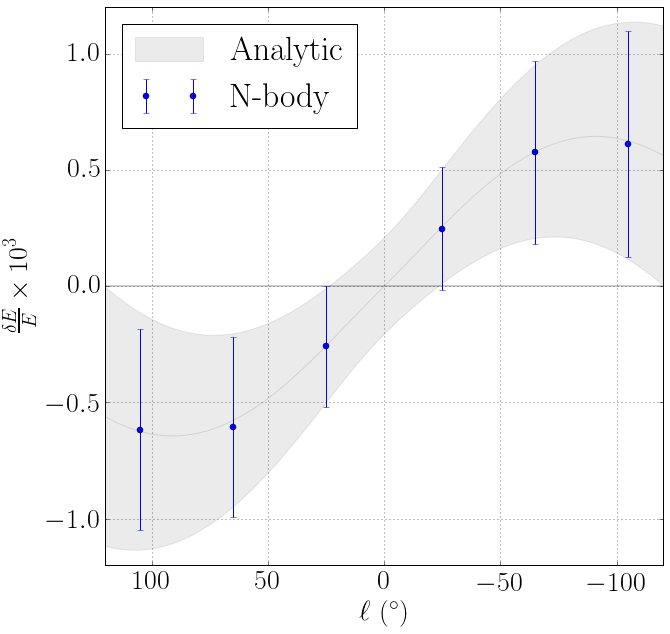
\includegraphics[width=1.0\columnwidth]{de_vs_l_filled.png}
\caption{Velocity spectroscopy of the Milky Way halo, giving the position of the observed line centroid due to sterile
	neutrino decay as a function of Galactic longitude $\ell$, with latitude $b=25^\circ$. This
	compares results as computed from an N-body simulation (Halo 374; see Section \ref{sec:simulations}) for the
	instrumental parameters of Micro-X against our analytic model (Section
	\ref{sec:theory}), showing good agreement.	
	Note that the error bars and shaded region represent the 1-$\sigma$ uncertainty
	in the energy of the line centroid, rather than the Doppler-broadened width of the line.}
\label{fig:de_vs_l}
\end{figure}

%\begin{figure}[h!]
%\centering
%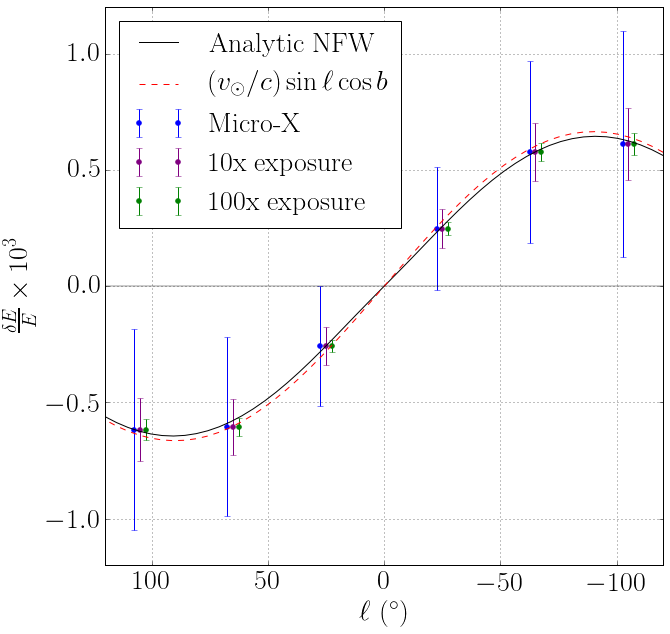
\includegraphics[width=1.0\columnwidth]{de_vs_l.png}
%\caption{Velocity spectroscopy of the Milky Way halo, giving the position of the observed line centroid due to sterile
	%neutrino decay as a function of Galactic longitude $\ell$, with latitude $b=25^\circ$. This
	%compares results as computed from an N-body simulation (Halo 374; see Section \ref{sec:simulations}) for the
	%instrumental parameters of Micro-X against our analytic model (Section
	%\ref{sec:theory}), showing good agreement.	
	%Note that the error bars here represent the 1-$\sigma$ uncertainty
	%in the energy of the line centroid, rather than the Doppler-broadened width of the line.}
%\label{fig:de_vs_l}
%\end{figure}

\begin{figure}[h!]
\centering
\begin{subfigure}[b]{1.0\columnwidth}
	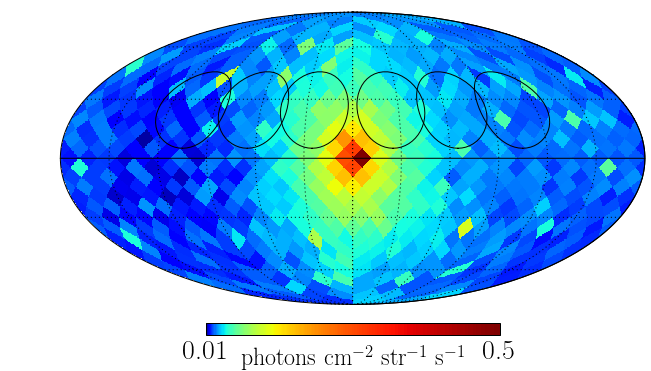
\includegraphics[width=\textwidth]{flux_map_374.png}
\subcaption{Flux.}
\end{subfigure}
\par\medskip
\begin{subfigure}[b]{1.0\columnwidth}
	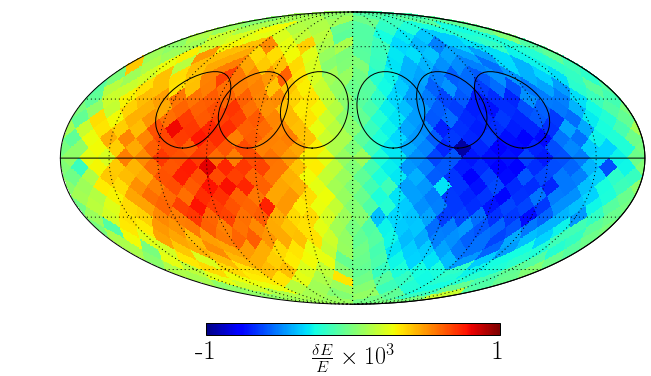
\includegraphics[width=\textwidth]{line_map_374.png}
\subcaption{Doppler-shifted line centroid.}
\end{subfigure}
\par\medskip
\begin{subfigure}[b]{1.0\columnwidth}
	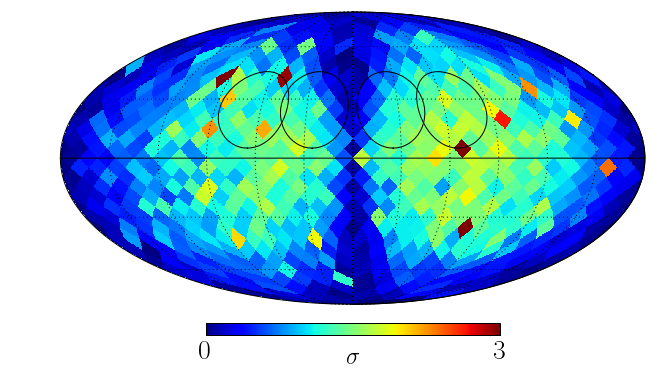
\includegraphics[width=\textwidth]{sigma_map_374.png}
\subcaption{Exclusion of the line centroid from $\delta E/E=0$.}
\end{subfigure}
\caption{Sky maps illustrating the principle of velocity spectroscopy. Top: The flux map. Middle:
	The dipole pattern in the line energy induced by our motion relative to the Milky Way halo.
	Bottom: The signicance of the detection of Doppler shifting of a dark matter decay line,
indicating the number of $\sigma$ by which $\delta E/E=0$ can be excluded for a Micro-X-like
observation. Black circles indicate the
FOV of Micro-X on the sky for the six pointings used in Figure \ref{fig:de_vs_l}. }
\label{fig:skymaps}
\end{figure}



%\subsection{Halo triaxiality}
%\label{sec:triaxiality}

\begin{figure}[h!]
\centering
\begin{subfigure}[b]{1.0\columnwidth}
	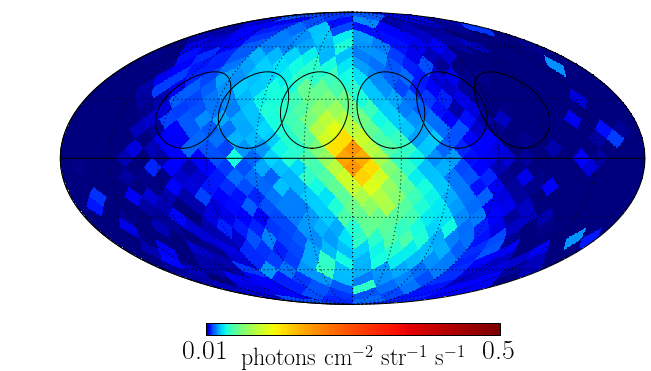
\includegraphics[width=\textwidth]{flux_map_800.png}
\end{subfigure}
\par\medskip
\begin{subfigure}[b]{1.0\columnwidth}
	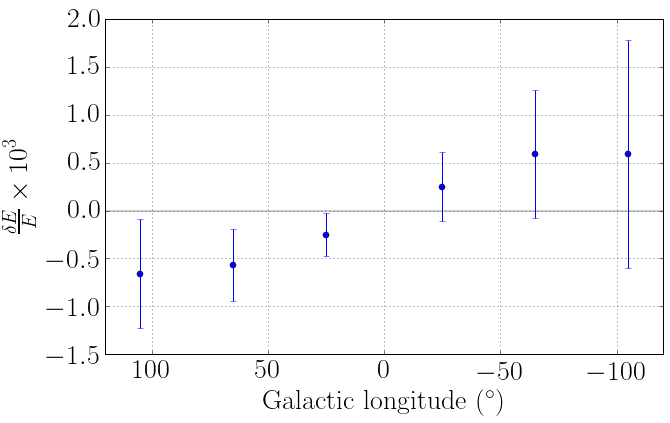
\includegraphics[width=\textwidth]{de_vs_l_800.png}
\end{subfigure}
\caption{Asymmetry of the Milky Way halo (here, Halo 800 with $b/a=$ and $c/a=$) could skew the significance of the
	observed signal to the east or west. Each field of view (black circles in the sky map) corresponds to a data point in
the lower plot. The gray shaded region indicates the $1\sigma$ uncertainties for the analytic model
derived from a spherical NFW profile fit to this halo.}
\label{fig:triax}
\end{figure}

%While this is not expected to 


% % % % % % % % % % % CONCLUSIONS % % % % % % % % % % % % % % % % % % % % % %
\section{Conclusions}
\label{sec:conclusions}

 
\vspace{-0.5 cm}
	
% % % % % % % % % % % % % % % % % % % % % % % % % % % % % % % % % % % % % %		

% % % % % % % % % % % % % % % %Acknowledgments % % % % % % % % % % % % % % %
\section*{Acknowledgments} 

Mark Lovell, Yao-Yuan Mao, Chris Davis.

% % % % % % % % % % % % % % % % % % % % % % % % % % % % % % % % % % % % % % % % %	

\newcommand{\mnras}[0]{M.N.R.A.S.}
\bibliographystyle{kp}
%\bibliography{Bibliography/references}	
\bibliography{references}	

\end{document}
